\documentclass[tikz,border=6pt]{standalone}
\usepackage{xcolor}
\usepackage{tikz}
\usetikzlibrary{arrows.meta,positioning,calc,fit,backgrounds,shapes.geometric}

\definecolor{panelblue}{HTML}{EAF2FB}
\definecolor{panelred}{HTML}{FCECEC}
\definecolor{panelgray}{HTML}{F4F6F8}
\definecolor{panelgreen}{HTML}{EAF7EF}
\definecolor{accentblue}{HTML}{377EB8}
\definecolor{accentred}{HTML}{D55E5E}
\definecolor{accentgreen}{HTML}{4DAA70}
\definecolor{textgray}{HTML}{555555}
\definecolor{linegray}{HTML}{6F7A86}
\definecolor{softgreen}{HTML}{2E7D32}
\definecolor{softorange}{HTML}{C25B12}

\usepackage{lmodern}
\SetSymbolFont{letters}{bold}{OML}{cmbr}{bx}{it}
\renewcommand{\familydefault}{\sfdefault}
\usepackage{sansmathfonts}

\begin{document}
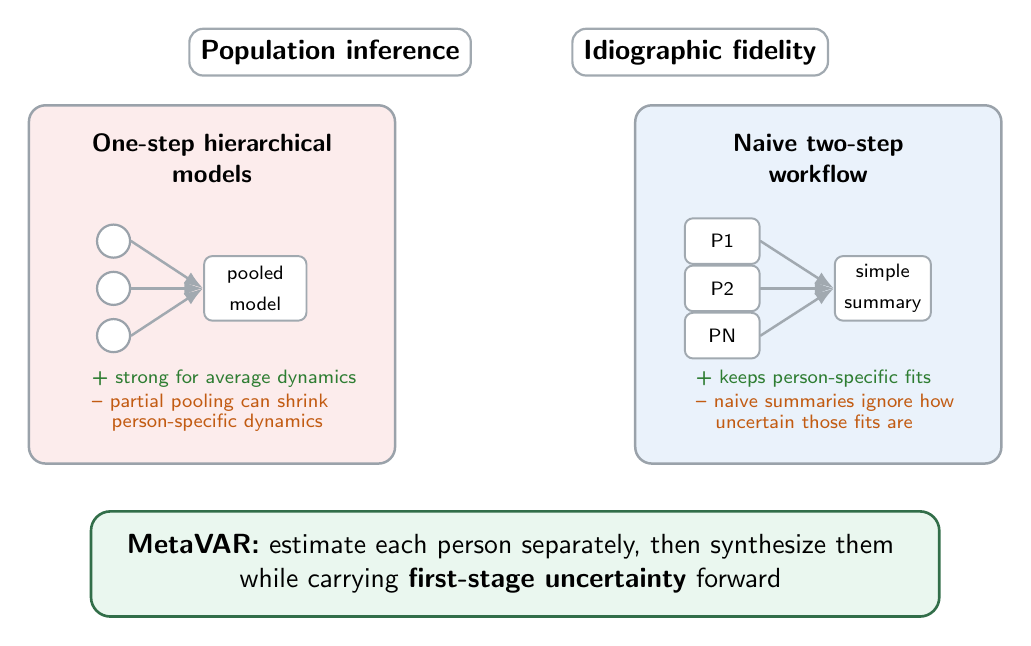
\begin{tikzpicture}[
    x=1cm,y=1cm,
    >=Latex,
    line cap=round,
    line join=round,
    panel/.style={draw=linegray!70, rounded corners=6pt, line width=0.9pt, minimum width=4.65cm, minimum height=4.55cm, inner sep=7pt, align=center},
    smallbox/.style={draw=linegray!65, rounded corners=3pt, line width=0.7pt, fill=white, inner sep=2.5pt, minimum width=0.95cm, minimum height=0.58cm, align=center},
    person/.style={circle, draw=linegray!70, line width=0.8pt, fill=white, minimum size=0.42cm, inner sep=0pt},
    iconlabel/.style={font=\scriptsize, text=textgray, align=center},
    paneltitle/.style={font=\bfseries\small, text=black, align=center},
    banner/.style={draw=accentgreen!65!black, fill=panelgreen, rounded corners=7pt, line width=0.95pt, inner sep=7pt, align=center},
    chip/.style={draw=linegray!65, fill=white, rounded corners=5pt, line width=0.8pt, inner sep=4pt, align=center},
    flow/.style={-{Latex[length=2.6mm,width=1.9mm]}, line width=0.95pt, draw=linegray!80},
    softflow/.style={-{Latex[length=2.4mm,width=1.7mm]}, line width=0.9pt, draw=linegray!65},
    positive/.style={font=\scriptsize, text=softgreen, align=left},
    negative/.style={font=\scriptsize, text=softorange, align=left},
    main/.style={font=\bfseries\small, text=black}
]

% Goal chips
\node[chip, minimum width=2.5cm] (goal1) at (3.35,2.95) {\textbf{Population inference}};
\node[chip, minimum width=2.5cm] (goal2) at (8.05,2.95) {\textbf{Idiographic fidelity}};
% \draw[flow, draw=linegray!60] (goal1.east) -- node[above, font=\scriptsize, text=textgray] {current workflows often force a trade-off} (goal2.west);

% Panels
\node[panel, fill=panelred]   (leftpanel)  at (1.85,0) {};
\node[panel, fill=panelblue]  (rightpanel) at (9.55,0) {};

% Left panel
\node[paneltitle] at ([yshift=1.60cm]leftpanel.center) {One-step hierarchical\\models};
\node[person] (lp1) at ([xshift=-1.25cm,yshift=0.55cm]leftpanel.center) {};
\node[person] (lp2) at ([xshift=-1.25cm,yshift=-0.05cm]leftpanel.center) {};
\node[person] (lp3) at ([xshift=-1.25cm,yshift=-0.65cm]leftpanel.center) {};
\node[smallbox, minimum width=1.3cm, minimum height=0.82cm] (lmodel) at ([xshift=0.55cm,yshift=-0.05cm]leftpanel.center) {\scriptsize pooled\\[-0.1em]\scriptsize model};
\draw[softflow] (lp1.east) -- (lmodel.west);
\draw[softflow] (lp2.east) -- (lmodel.west);
\draw[softflow] (lp3.east) -- (lmodel.west);
\node[positive, anchor=west] at ([xshift=-1.65cm,yshift=-1.20cm]leftpanel.center) {\textbf{+} strong for average dynamics};
\node[negative, anchor=west] at ([xshift=-1.65cm,yshift=-1.50cm]leftpanel.center) {\textbf{--} partial pooling can shrink};
\node[negative, anchor=west] at ([xshift=-1.40cm,yshift=-1.75cm]leftpanel.center) {person-specific dynamics};

% Right panel
\node[paneltitle] at ([yshift=1.60cm]rightpanel.center) {Naive two-step\\workflow};
\node[smallbox] (rb1) at ([xshift=-1.22cm,yshift=0.55cm]rightpanel.center) {\scriptsize P1};
\node[smallbox] (rb2) at ([xshift=-1.22cm,yshift=-0.05cm]rightpanel.center) {\scriptsize P2};
\node[smallbox] (rb3) at ([xshift=-1.22cm,yshift=-0.65cm]rightpanel.center) {\scriptsize PN};
\node[smallbox, minimum width=1.22cm, minimum height=0.82cm] (ravg) at ([xshift=0.82cm,yshift=-0.05cm]rightpanel.center) {\scriptsize simple\\[-0.1em]\scriptsize summary};
\draw[softflow] (rb1.east) -- (ravg.west);
\draw[softflow] (rb2.east) -- (ravg.west);
\draw[softflow] (rb3.east) -- (ravg.west);
\node[positive, anchor=west] at ([xshift=-1.68cm,yshift=-1.20cm]rightpanel.center) {\textbf{+} keeps person-specific fits};
\node[negative, anchor=west] at ([xshift=-1.68cm,yshift=-1.50cm]rightpanel.center) {\textbf{--} naive summaries ignore how};
\node[negative, anchor=west] at ([xshift=-1.43cm,yshift=-1.75cm]rightpanel.center) {uncertain those fits are};

% MetaVAR box
\node[banner, minimum width=10.7cm] (bottom) at (5.70,-3.55) {
    \begin{tabular}{c}
    \textbf{MetaVAR:} estimate each person separately, then synthesize them \\
    while carrying \textbf{first-stage uncertainty} forward
    \end{tabular}
};

% \draw[flow, draw=accentgreen!65!black] ([yshift=-0.05cm]leftpanel.south east) .. controls +(0.9,-0.7) and +(-2.1,1.1) .. ([xshift=-1.1cm]bottom.north);
% \draw[flow, draw=accentgreen!65!black] ([yshift=-0.05cm]rightpanel.south west) .. controls +(-0.9,-0.7) and +(2.1,1.1) .. ([xshift=1.1cm]bottom.north);

% \node[iconlabel] at ([yshift=-1.08cm]bottom.south) {preserve idiographic first-stage estimation \quad + \quad support valid population-level inference};

\end{tikzpicture}
\end{document}
